\chapter{Базис полиномов Лежандра}\label{sec:legendre}

Базис представляет собой набор n первых полиномов Лежандра:
$$P_n(z)=\frac{1}{2^n n!}\frac{d^n}{dz^n}(z^2-1)^n$$
Такая система ортогональна на отрезке [-1,1], но этот отрезок может быть переопределен заменой переменной в полиномах.
\begin{figure}[h!]
	\begin{minipage}[h]{0.49\linewidth}
		\center{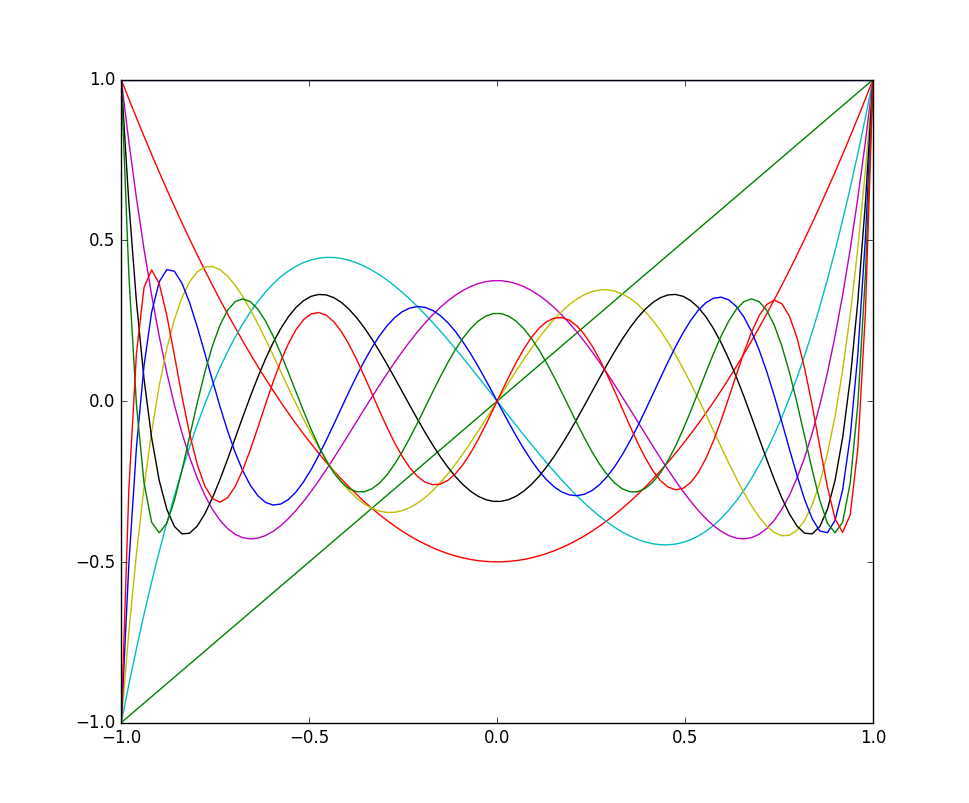
\includegraphics[scale=0.25]{figure_1}}
		\center{\caption{Базисные функции}}
	\end{minipage}
\hfill
	\begin{minipage}[h]{0.49\linewidth}
		\center{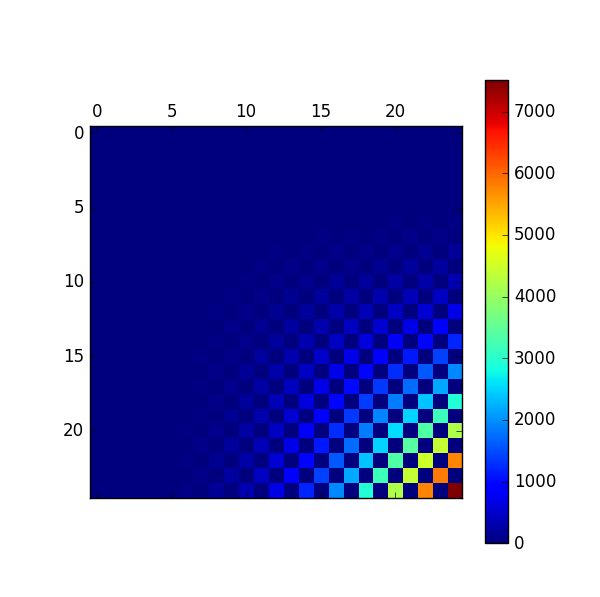
\includegraphics[scale=0.4]{figure_2}}
		\caption{Матрица $\Omega$}
	\end{minipage}
\label{ris:image1}
\end{figure}
Производится разложение функции в ряд вида
$$f(\mu)=a_0 P_0 (\mu) + a_1 P_1 (\mu) + ... +  a_n P_n (\mu),$$
$-1 < \mu <1 .$
Коэффициенты разлодения определяются как:
$$a_m = \frac{1}{2}(2m+1)\int\limits_{-1}^{1}f(\mu)P_m (\mu)d\mu .$$
Такая система ортогональна на отрезке [-1,1], но этот отрезок может быть переопределен заменой переменной в полиномах.

\section{Базис Фурье}\label{sec:fourier}

В качестве Фурье базиса используется тригонометрический ряд Фурье \{$\sin nx, \cos nx$\}.
Разложение функции по базису производится по формулам:
$$f(x)=\frac{a_0}{2} + \sum^{\infty}_{n=1} (a_n \cos nx + b_n \sin nx)$$
где
$$a_0= \frac{1}{\pi}\int\limits_{-\pi}^{\pi}f(x)dx,$$
$$a_n= \frac{1}{\pi}\int\limits_{-\pi}^{\pi}f(x)\cos(nx)dx,$$
$$b_n= \frac{1}{\pi}\int\limits_{-\pi}^{\pi}f(x)\sin(nx)dx.$$

\section{B-сплайны}\label{sec:spline}

B-сплайны (базисные сплайны) --- базисные функции, использующиеся для апроксимации ломаных. Кривая, построенная на основе B-сплайн-базиса, описывается следующим образом:
$$\vec{p}(t)=\sum^{n}_{i=0} \vec{P_i}N_{ik} (t),$$
где $\vec{p}(t)$ --- радиус-вектор точек на кривой, $\vec{P_i}$ --- вершины аппроксимируемой ломаной (всего вершин n+1), а $N_{ik} (t)$ --- весовая функция ш-й нормальзованноый B-сплайн базисной кривой порядка k (т.е. степени k-1), задаваемая рекурентными соотношениями:
\begin{equation*}
N_{i1} = 
 \begin{cases}
   1, &\text{если $x_i \leq t \leq x_{i-1},$}\\
   0, &\text{если $t \notin (x_i, x_{i-1})$}
 \end{cases}
\end{equation*}
$$ N_{ik} (t) = \frac{(t-x_i)N_{i,k-1}(t)}{x_{i+k-1} - x_i} - \frac{(x_{i+k}-t)N_{i+1,k-1}(t)}{x_{i+k} - x_{i+1}} .$$
Здесь $x_i$ --- элементы узлового вектора, а t – параметр, изменяю­щийся в диапазоне от 0 до $t_{max}=(n – k+2)$.
B-сплайн-кривая является полиномом степени (k–1) на каждом интервале $(x_i, x_{i+1})$, и все ее производные до (k–2)-го порядка включительно непрерывны вдоль всей кривой. То есть эта кривая представляет собой сплайн-функцию порядка k (степени k–1).
